\section{A Lefschetz-type theorem for quasimaps} \label{Section quasimap mirror theorem}

In \cite{Ga-MF} Gathmann applies his recursion formula for relative stable maps to obtain a new proof of the mirror theorem for hypersurfaces \cite{Givental-mirror} \cite{LLY1}. This can be viewed as a quantum Lefschetz formula, expressing stable map invariants of $Y$ in terms of those of $X$.

In this section we carry out a similar computation in the quasimap setting, using the recursion found in Theorem \ref{Theorem general recursion} above. We work with generating functions for $2$-pointed quasimap invariants (the minimal number of markings, due to the strong stability condition). The absence of rational tails in the quasimap moduli space makes the quasimap recursion much simpler than Gathmann's. We obtain a \emph{Lefschetz-type theorem for quasimap invariants} (Theorem \ref{Theorem Quantum Lefschetz}), that is, a formula which expresses quasimap invariants of $Y$ in terms of those of $X$. This is the quasimap analogue of the quantum Lefschetz formula in Gromov--Witten theory.

Our formula can be viewed as a special case of \cite[Corollary 5.5.1]{CF-K-wallcrossing}, and thus as a relation between certain residues of the $\Gm$-action on spaces of $0$-pointed and $1$-pointed parametrised quasimaps to $Y$. Some of the consequences of this formula are explored in \cite[Section 5.5]{CF-K-wallcrossing}; for instance, it follows in the semipositive case that all primary $\epsilon$-quasimap invariants with a fundamental class insertion can be expressed in terms of $2$-pointed invariants.

\subsection{Setup} \label{Subsection setup}
As before, we let $X=X_{\Sigma}$ be a smooth projective toric variety and $i \colon Y \hookrightarrow X$ a smooth very ample hypersurface. We also make the following two assumptions:
\begin{enumerate}
\item \emph{$Y$ is semi-positive}: $-K_Y$ is nef;
\item \emph{$Y$ contains all curve classes}: the map $i_* : \Achow_1(Y) \to \Achow_1(X)$ is surjective.
\end{enumerate}
By adjunction, $-K_X$ pairs strictly positively with every curve class coming from $Y$, hence with every curve class by Assumption (2). Thus $-K_X$ is ample, or in other words, $X$ is Fano\footnote{Kleiman's criterion says that a divisor $D$ is ample if and only if $D \cdot C > 0$ for every curve class $C$ in the closure of the effective cone. But since $X$ is a toric variety the effective cone is finitely generated in $\Achow_1(X)$, hence is closed in $\Achow_1(X)_{\mathbb{R}}$ as it is a finite intersection of half-spaces. So we only need to check $D \cdot C > 0$ for every effective curve class.}. Also note that if $\dim X \geq 3$ then Assumption (2) always holds, due to the classical Lefschetz hyperplane theorem; on the other hand if $\dim X = 2$ then Assumption (2) forces $X$ to be $\PP^2$.

We fix a homogeneous basis $\eta_0, \ldots, \eta_k$ for $\HH^*(X) = \HH^*(X,\QQ)$ and let $\eta^0, \ldots, \eta^k$ denote the dual basis with respect to the Poincar\'e pairing. Without loss of generality we may suppose that $\eta^0=\mathbbm 1_X$ and $\eta^1=[Y]$. We get an induced basis $\rho_1=i^*\eta_1, \ldots, \rho_k = i^* \eta_k$ for $i^*\HH^*(X)$. Notice that $\rho_0 = i^* \eta_0 = i^* [\pt_X] = 0$, $\rho_1 = i^* \eta_1 = [\pt_Y]$.  We can extend the $\rho_i$ to a basis $\rho_1, \ldots, \rho_l$ for $\HH^*(Y)$ by adding $\rho_{k+1}\ldots,\rho_{l}$. Let $\rho^1, \ldots, \rho^l$ denote the dual basis; notice that $\rho^i$ is \emph{not} equal to $i^* \eta^i$ (they do not even have the same degree!).  Note also that $\rho^1 = \mathbbm{1}_Y$.

\subsection{Generating functions for quasimap invariants}
As with many results in enumerative geometry, the quasimap Lefchetz formula is most conveniently stated in terms of generating functions. Here we define several such generating functions for the absolute quasimap invariants of $X$ and $Y$.  We work with two marked points since this is the minimum number required in order for the quasimap space to be nonempty. However since we only take insertions at the first marking we would like to think of these, morally speaking, as $1$-pointed invariants (in Gromov--Witten theory the corresponding statement is literally true, due to the string equation).

For any smooth projective toric variety\footnote{Or more generally any space for which the quasimap invariants are defined, for instance a smooth hypersurface in a toric variety.} $X$ and any effective curve class $\beta\in \HH_2^+(X)$, we define
\begin{align*} S_0^X(z,\beta) & =(\ev_1)_*\left(\frac{1}{z-\psi_1} \virt{\Q{0}{2}{X}{\beta}}\right) 
\intertext{and}
S_0^X(z,q) &=\sum_{\beta\geq 0} q^\beta S_0^X(z,\beta)\end{align*}
where by convention $S_0^X(z,0)= \mathbbm 1_X$, and $q$ is a Novikov variable. These are generating functions for quasimap invariants of $X$ which take values in $\HH^*(X)$.

The same definition applies to $Y$. However, sometimes we may wish to consider only insertions of cohomology classes coming from $X$. These are the so-called \emph{restricted quasimap invariants}, and the corresponding generating function is defined as
\begin{equation*} \tilde{S}^Y_0(z,\beta) = (\ev_1)_* \left( \dfrac{1}{z-\psi_1} \virt{\Q{0}{2}{Y}{\beta}} \right) \end{equation*}
where crucially $\ev_1$ is viewed as \emph{mapping to $X$} instead of to $Y$. Thus $\tilde{S}^Y_0(z,\beta)$ takes values in $\HH^*(X)$ and involves only quasimap invariants of $Y$ with insertions coming from $i^*\HH^*(X)$; this is in contrast to $S^Y_0(z,\beta)$, which takes values in $\HH^*(Y)$ and involves quasimap invariants of $Y$ with arbitrary insertions. As earlier, we can also define $\tilde{S}_0^Y(z,q)$.

Now, since $X$ and $Y$ are smooth, we may use Poincar\'{e} duality to define a push-forward map on cohomology, $i_* \colon \HH^k(Y) \to \HH^{k+2}(X)$.

\begin{lemma} $i_* S^Y_0(z,\beta) = \tilde{S}^Y_0(z,\beta)$. \end{lemma}
\begin{proof} This follows from functoriality of cohomological push-forwards and the fact that we have a commuting triangle:
\bcd
\Q{0}{2}{Y}{\beta} \ar[rr,"\ev_1"] \ar[rd,"\ev_1" left=0.2cm] & & Y \ar[ld,"i"] \\
& X & 
\ecd
Let us spell this out explicitly, in order to help familiarise the reader with the generating functions involved. First, it is easy to see from the projection formula that:
\begin{align*} i_* \rho^i =
\begin{cases} \eta^i \qquad \text{for $i = 1, \ldots, k$} \\
0 \qquad \text{\ for $i = k+1, \ldots, l$} \end{cases} \end{align*}
Now, we can write $S_0^Y(z,\beta)$ as:
\begin{equation*} S_0^Y(z,\beta) = \sum_{i=1}^l \left\langle \dfrac{\rho_i}{z-\psi_1} , \mathbbm{1}_Y \right\rangle_{0,2,\beta}^Y  \rho^i \end{equation*}
Thus applying $i_*$ gives
\begin{align*} i_* S_0^Y(z,\beta)  = \sum_{i=1}^l \left\langle \dfrac{\rho_i}{z-\psi_1} , \mathbbm{1}_Y \right\rangle_{0,2,\beta}^Y   i_* \rho^i
= \sum_{i=1}^k \left\langle \dfrac{\eta_i}{z-\psi_1}, \mathbbm{1}_X \right\rangle_{0,2,\beta}^Y   \eta^i = \tilde{S}_0^Y(z,\beta) \end{align*}
as claimed. \end{proof}

\subsection{Quasimap Lefschetz formula} We now turn to our main result: a formula expressing the generating function $\tilde{S}_0^Y(z,q)$ for restricted quasimap invariants of $Y$ in terms of the quasimap invariants of $X$.

\begin{thm} \label{Theorem Quantum Lefschetz}
Let $X$ and $Y$ be as above. Then
\begin{equation}\label{eqn:mirror}
\dfrac{\sum_{\beta\geq 0} q^\beta\prod_{j=0}^{Y\cdot\beta}(Y+jz)S_0^X(z,\beta)}{P_0^X(q)}= \tilde{S}_0^Y(z,q)
\end{equation}
where:
\begin{align*}
 P_0^X(q) % & = 1 + \sum_{\substack{\beta>0 \\ K_Y\cdot\beta=0}} q^\beta (Y\cdot\beta) \langle [\pt_Y],\mathbbm 1_{X}\rangle_{0,(Y\cdot\beta,0),\beta}^{X|Y} \\
            & = 1 + \sum_{\substack{\beta>0 \\ K_Y\cdot\beta=0}} q^\beta(Y\cdot\beta)!\langle [\pt_X] \psi_1^{Y\cdot\beta-1} ,\mathbbm 1_{X}\rangle_{0,2,\beta}^X
\end{align*}
Notice that $P_0^X(q)$ depends not only on $X$ but also on the divisor class of $Y$ in~$X$; the superscript is supposed to indicate that the definition only involves quasimap invariants of $X$.
\end{thm}

\begin{proof}
For $m = 0, \ldots, Y \cdot \beta$, define the following generating function for $2$-pointed relative quasimap invariants
 \[
  S_{0,(m)}^{X|Y}(z,\beta)=(\ev_1)_*\left(\frac{1}{z-\psi_1}\virt{\Q{0}{(m,0)}{X|Y}{\beta}}\right)
 \]
where we view $\ev_1$ as mapping to $X$.  Note that  $S_{0,(0)}^{X|Y}(z,\beta) = S_0^X(z, \beta)$. Also define the following generating function for ``comb loci invariants''
\[
 T_{0,(m)}^{X|Y}(z,\beta)=(\ev_1)_*\left(m \virt{\Q{0}{(m,0)}{X|Y}{\beta}}+\frac{1}{z-\psi_1} \virt{\mathcal{D}^{\mathcal{Q}}_{(m,0),1}(X|Y,\beta)} \right)
\]
where again we view $\ev_1$ as mapping to $X$. As in \cite[Lemma 1.2]{Ga-MF}, it follows from Theorem \ref{Theorem general recursion} that
\begin{equation}
 (Y+mz) S_{0,(m)}^{X|Y}(z,\beta) = S_{0,(m+1)}^{X|Y}(z,\beta)+ T_{0,(m)}^{X|Y}(z,\beta)
\end{equation}
and we can apply this repeatedly to obtain:
\begin{equation} \label{eqn:G}
\prod_{j=0}^{Y\cdot\beta}(Y+jz) S_0^X(z,\beta) = \sum_{m=0}^{Y\cdot\beta}\prod_{j=m+1}^{Y\cdot\beta}(Y+jz)T_{0,(m)}^{X|Y}(z,\beta)
\end{equation}
We now examine the right-hand side in detail. By definition, $T_{0,(m)}^{X|Y}(z,\beta)$ splits into two parts: those terms coming from the relative space and those terms coming from the comb loci.

Let us first consider the contribution of the comb loci. Since there are only two marked points and the first is required to lie on the internal component of the comb, it follows from the strong stability condition that there are only two options: a comb with zero teeth or a comb with one tooth.

First consider the case of a comb with zero teeth. The moduli space is then $\Q{0}{2}{Y}{\beta}$ and we require that $Y \cdot \beta = m$. Thus this piece only contributes to $T_{0,(Y\cdot\beta)}^{X|Y}(z,\beta)$, and the contribution is:
\begin{equation*} \sum_{i=1}^k \left\langle \dfrac{\rho_i}{z-\psi_1}, \mathbbm{1}_Y \right\rangle_{0,2,\beta}^Y \eta^i \end{equation*}

Next consider the case of a comb with one tooth. Let $\beta^{(0)}$ and $\beta^{(1)}$ denote the curve classes of the internal and external components, respectively, and let $m^{(1)}$ be the contact order of the external component with $Y$. The picture is as follows
\begin{center}
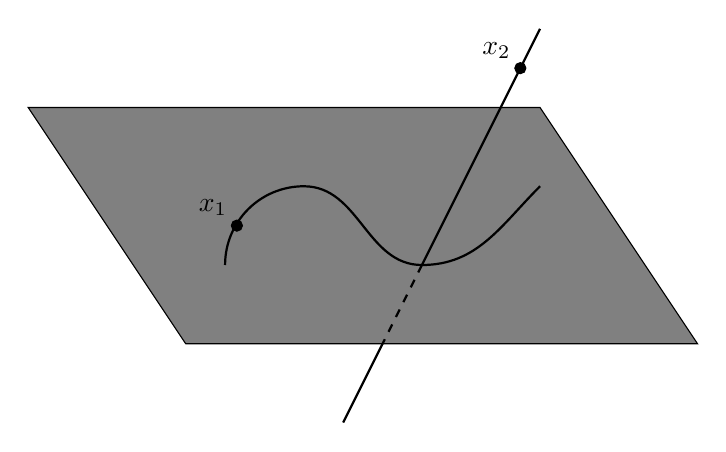
\begin{tikzpicture}
  \draw [fill=gray] (-.5,-1) -- (6,-1) -- (4,2) -- (-2.5,2) -- (-.5,-1);
  \draw [thick] (0,0) to [out=90,in=180] (1,1) to [out=0,in=180] (2.5,0) to [out=0,in=-135] (4,1);
  \draw [thick] (2.5,0) to (4,3);
  \draw [thick,dashed] (2.5,0) to (2,-1);
  \draw [thick] (2,-1) -- (1.5,-2);
  \draw [fill] (3.75,2.5) circle [radius=2pt] node[above left]{$x_2$};
  \draw [fill] (.15,.5) circle [radius=2pt] node[above left]{$x_1$};
 \end{tikzpicture}
\end{center}
and the invariants which contribute take the form
\begin{equation*} \bigg\langle \dfrac{\rho_i}{z-\psi_1},\rho^h\bigg\rangle_{0,2,\beta^{(0)}}^Y \bigg\langle \rho_h, \mathbbm 1_{X}\bigg\rangle_{0,(m^{(1)},0),\beta^{(1)}}^{X|Y} \end{equation*}
for $i = 1, \ldots, k$ and $h = 1, \ldots, l$. By computing dimensions, we find
\begin{align*}
0\leq \codim \rho^h &= \dim Y-\codim \rho_h \\
&= \dim Y-\vdim \Q{0}{(m^{(1)},0)}{X|Y}{\beta^{(1)}} \\
&= \dim Y-(\dim X-3-K_{X}\cdot \beta^{(1)}+2-m^{(1)})\\
&= K_Y \cdot \beta^{(1)} - Y \cdot \beta^{(1)}+m^{(1)} \\
&\leq 0
\end{align*}
where the final equality follows from adjunction and the final inequality holds because $-K_Y$ is nef and $m^{(1)}\leq Y \cdot \beta_1$. This shows that the only non-trivial contributions come from curve classes $\beta^{(1)}$ such that $K_Y \cdot \beta^{(1)}=0$, and that in this case the order of tangency must be maximal, i.e. $m^{(1)}=Y \cdot \beta^{(1)}$. Furthermore we must have $\codim \rho^h = 0$ and so $\rho^h = \rho^1 = \mathbbm{1}_Y$ which implies $\rho_h = \rho_1 = [\pt_Y]$. Finally since $m^{(1)}=Y \cdot \beta^{(1)}$ we have
\begin{equation*} m = Y \cdot \beta^{(0)}+m^{(1)}=Y \cdot (\beta^{(0)} + \beta^{(1)}) = Y \cdot \beta \end{equation*}
and so again this piece only contributes to $T_{0,(Y\cdot\beta)}^{X|Y}(z,\beta)$, and the contribution is:
\begin{equation*} \sum_{i=1}^k \left( \sum_{\substack{0 < \beta^{(1)} < \beta \\ K_Y \cdot \beta^{(1)}=0}} (Y \cdot \beta^{(1)}) \bigg\langle \dfrac{\rho_i}{z-\psi_1}, \mathbbm{1}_Y \bigg\rangle_{0,2,\beta-\beta^{(1)}}^Y \bigg\langle \rho_1, \mathbbm{1}_X \bigg\rangle_{0,(Y \cdot \beta^{(1)},0),\beta^{(1)}}^{X|Y} \right) \eta^i \end{equation*}
where the $Y \cdot \beta^{(1)}$ factor comes from the weighting on the virtual class of the comb locus. Finally, we must examine the terms of $T_{0,(m)}^{X|Y}(z,\beta)$ coming from:
\begin{equation*}\ev_{1*}(m\virt{\Q{0}{(m,0)}{X|Y}{\beta}})\end{equation*} 
Notice that we only have insertions from $i^*\HH^*(X) \subseteq \HH^*(Y)$, since $\ev_1$ is viewed as mapping to $X$. On the other hand
\begin{align*} \vdim \Q{0}{(m,0)}{X|Y}{\beta} & = \dim X-3 -K_X \cdot \beta +2-m & \\
& = \dim X - 1 -K_Y \cdot \beta + Y \cdot \beta - m \ \ & \text{by adjunction} \\
& \geq \dim X - 1 + Y\cdot\beta - m \ \ & \text{since $-K_Y$ is nef} \\
& \geq \dim X - 1 \ \ & \text{since $m \leq Y \cdot \beta$} \end{align*}
where in the second line we have applied the projection formula to $i$, and thus have implicitly used Assumption (2), discussed in \S \ref{Subsection setup}; namely that every curve class on $X$ comes from a class on $Y$.

Consequently the only insertions that can appear are those of dimension $0$ and $1$. However, the restriction of the $0$-dimensional class $\eta_0 = [\pt_X]$ to $Y$ vanishes, as do the restrictions of all $1$-dimensional classes except for $\eta_1$ (by the definition of the dual basis, since $\eta^1 = Y$). Thus the only insertion is $i^*\eta_1=\rho_1=[\pt_Y]$, and since $\eta^1$ has dimension $1$ all the inequalities above must actually be equalities. Thus we only have a contribution if $-K_Y \cdot \beta = 0$ and $m = Y \cdot \beta$. The contribution to $T_{0,(Y\cdot\beta)}^{X|Y}(z,\beta)$ in this case is:
\begin{equation*} (Y \cdot \beta) \langle \rho_1 , \mathbbm{1}_X \rangle_{0,(Y \cdot \beta,0),\beta}^{X|Y} \eta^1 \end{equation*}

Thus we have calculated $T_{0,(m)}^{X|Y}(z,\beta)$ for all $m$; substituting into equation \eqref{eqn:G} we obtain
\begin{align*} \prod_{j=0}^{Y \cdot \beta} (Y + jz) & S_0^X(z,\beta) = T_{0,(Y\cdot\beta)}^{X|Y}(z,\beta) \\
= \ & \sum_{i=1}^k \left\langle \dfrac{\rho_i}{z-\psi_1}, \mathbbm{1}_Y \right\rangle_{0,2,\beta}^Y \eta^i + \\
& \sum_{i=1}^k \left( \sum_{\substack{0 < \beta^{(1)} < \beta \\ K_Y \cdot \beta^{(1)}=0}} (Y \cdot \beta^{(1)}) \bigg\langle \dfrac{\rho_i}{z-\psi_1}, \mathbbm{1}_Y \bigg\rangle_{0,2,\beta-\beta^{(1)}}^Y \bigg\langle \rho_1, \mathbbm{1}_X \bigg\rangle_{0,(Y \cdot \beta^{(1)},0),\beta^{(1)}}^{X|Y} \right) \eta^i + \\
& (Y \cdot \beta) \langle \rho_1 , \mathbbm{1}_X \rangle_{0,(Y \cdot \beta,0),\beta}^{X|Y} \eta^1
\end{align*}
where the third term only appears if $K_Y \cdot \beta=0$. We can rewrite this as:
\begin{align*} \prod_{j=0}^{Y \cdot \beta} (Y + jz) & S_0^X(z,\beta) \\
& = \tilde{S}_0^Y(z,\beta) + \sum_{\substack{0 < \beta^{(1)} \leq \beta \\ K_Y \cdot \beta^{(1)}=0}} \left( (Y \cdot \beta^{(1)}) \bigg\langle \rho_1, \mathbbm{1}_X \bigg\rangle_{0,(Y \cdot \beta^{(1)},0),\beta^{(1)}}^{X|Y} \right) \tilde{S}_0^Y(z,\beta-\beta^{(1)})
\end{align*}
It is now clear from the expression above that equation \eqref{eqn:mirror} in the statement of Theorem \ref{Theorem Quantum Lefschetz} holds, with:
\begin{equation*} P_0^X(q) = 1 + \sum_{\substack{\beta>0 \\ K_Y\cdot\beta=0}} q^\beta (Y\cdot\beta) \langle \rho_1,\mathbbm 1_{X}\rangle_{0,(Y\cdot\beta,0),\beta}^{X|Y} \end{equation*}
To complete the proof it thus remains to show that:
\begin{equation*} P_0^X(q) = 1 + \sum_{\substack{\beta>0 \\ K_Y\cdot\beta=0}} q^\beta(Y\cdot\beta)!\langle\psi_1^{Y\cdot\beta-1} [\pt_X],\mathbbm 1_{X}\rangle_{0,2,\beta}^X \end{equation*}
The aim therefore is to express the relative invariants
\begin{equation*} \langle \rho_1 , \mathbbm{1}_X \rangle_{0,(Y\cdot\beta,0),\beta}^{X|Y} \end{equation*}
in terms of absolute invariants of $X$. Unsurprisingly, we once again do this by applying Theorem \ref{Theorem general recursion}. We have:
\begin{align*} \virt{\Q{0}{(Y \cdot \beta,0)}{X|Y}{\beta}} = \ & ((Y\cdot\beta-1)\psi_1+\ev_1^*Y) \virt{\Q{0}{(Y\cdot\beta-1,0)}{X|Y}{\beta}} \ - \\
& \virt{\mathcal{D}_{(Y\cdot\beta-1,0),1}^{\mathcal Q}(X|Y,\beta)} \end{align*}
We begin by examining the contributions from the comb loci. As before, we have the contributions coming from combs with $0$ teeth and combs with $1$ tooth. The former contributions take the form
\begin{equation*} \langle \rho_1 , \mathbbm{1}_Y \rangle_{0,2,\beta}^Y \end{equation*}
which vanish because $\vdim{\Q{0}{2}{Y}{\beta}} = \dim Y -1 -K_Y\cdot\beta = \dim Y -1$ whereas the insertion has codimension $\dim Y$. On the other hand, the latter contributions take the form
\begin{equation*} \langle \rho_1 ,\rho^h\rangle_{0,2,\beta^{(0)}}^Y \langle \rho_h,\mathbbm 1_{X}\rangle_{0,(Y\cdot(\beta-\beta^{(0)})-1,0),\beta-\beta^{(0)}}^{X|Y}\end{equation*}
and these must also vanish since:
\begin{align*} \codim \rho^h & = \dim Y - \codim \rho_h \\
& = \dim Y - \vdim \Q{0}{(Y\cdot(\beta-\beta^{(0)})-1,0)}{X|Y}{\beta-\beta^{(0)}} \\
& = \dim Y - (\dim X - 3 - K_X \cdot (\beta - \beta^{(0)}) + 2 - Y \cdot (\beta - \beta^{(0)}) + 1) \\
&= -1 + K_X \cdot (\beta-\beta^{(0)}) + Y \cdot (\beta-\beta^{(0)}) \\
& = -1 + K_Y\cdot(\beta-\beta^{(0)}) \\
& \leq -1
\end{align*}
Thus the comb loci do not contribute at all. Applying this recursively (the same argument as above shows that we never get comb loci contributions), we find that
\begin{align*}
(Y\cdot\beta)\langle \rho_1 ,\mathbbm 1_{X}\rangle_{0,(Y\cdot\beta,0),\beta}^{X|Y} & = (Y\cdot\beta) \langle \eta_1 \prod_{j=0}^{Y\cdot\beta-1}(Y+j\psi_1) , \mathbbm{1}_X \rangle_{0,2,\beta}^X \\
& = (Y\cdot\beta)!\langle[ \pt_X]\psi_1^{Y\cdot\beta-1},\mathbbm 1_X\rangle_{0,2,\beta}^X
\end{align*}
where the second equality holds because $Y\cdot\eta_1=\eta^1 \cdot \eta_1 = [\pt_X]$ and $Y^2\cdot\eta_1=0$. This completes the proof of Theorem \ref{Theorem Quantum Lefschetz}. \end{proof}

\begin{cor}
 If $Y$ is Fano then there is no correction term:
\begin{equation*} \sum_{\beta\geq 0} q^\beta\prod_{j=0}^{Y\cdot\beta}(Y+jz)S_0^X(z,\beta) = \tilde{S}_0^Y(z,q) \end{equation*}
\end{cor}

\begin{cor}
Let $Y = Y_5 \subseteq  X = \PP^4$ be the quintic three-fold. Then
\begin{equation*} \tilde{S}_0^{Y_5}(z,q)=\dfrac{I_{\text{sm}}^{Y_5}(z,q)}{P(q)} \end{equation*}
where
\begin{equation*} I_{\text{sm}}^{Y_5}(z,q)=5H+\sum_{d>0}\frac{\prod_{j=0}^{5d}(H+jz)}{\prod_{j=0}^{d}(H+jz)^5} \ q^d \end{equation*}
and:
\begin{equation*} P(q)=1+\sum_{d>0}\frac{(5d)!}{(d!)^5}q^d \end{equation*}
\end{cor}
\begin{proof} Apply Theorem \ref{Theorem Quantum Lefschetz} and use the fact that the quasimap invariants of $\PP^4$ coincide with the Gromov--Witten invariants, which are well-known from mirror symmetry. \end{proof}

\begin{remark}
Theorem \ref{Theorem Quantum Lefschetz} agrees with \cite[Theorem~1]{CZ-mirror} when $X$ is a projective space.
\end{remark}

\subsection{Comparison with the work of Ciocan-Fontanine and Kim}
Here we briefly explain how to compare our Theorem \ref{Theorem Quantum Lefschetz} to a formula obtained by Ciocan-Fontanine and Kim. We assume that the reader is familiar with the paper \cite{CF-K-wallcrossing}, in particular \S4 and \S5. There they introduce (in the more general context of $\epsilon$-stable quasimaps) the following generating functions for quasimap invariants of $Y$:
\begin{enumerate}
\item The \emph{$J^{\epsilon}$-function}
\begin{equation*} J^\epsilon({\bf t}, z)=\sum_{m\geq 0,\beta\geq 0} \dfrac{q^\beta}{m!} (\ev_\bullet)_*\left( \prod_{i=1}^m \ev_i^*({\bf t}) \cap\operatorname{Res}_{F_0} \virt{\QGe{0}{m}{Y}{\beta}} \right) \end{equation*}
for $\mathbf{t} \in \HH^*(X)$. Here $\QGe{0}{m}{Y}{\beta}$ is the moduli space of $\epsilon$-stable  quasimaps with a parametrised component, $F_0$ is a certain fixed locus of the natural $\Gm$-action on this space, and $\ev_\bullet$ is the evaluation at the point $0 \in \PP^1$ on the parametrised component. $\operatorname{Res}_{F_0}$ is the residue of the virtual class, i.e. the virtual class of the fixed locus divided by the Euler class of the virtual normal bundle (see \cite{GraberPandharipande} for details on virtual localisation). The variable $z$ is the $\Gm$-equivariant parameter.
\item The \emph{$S^\epsilon$-operator}
\begin{equation*}
 S^\epsilon(\mathbf{t},z)(\gamma)=\sum_{m\ge 0,\beta\ge 0}\frac{q^\beta}{m!} 
(\ev_1)_*\left( \dfrac{\ev_2^*(\gamma) \cdot \prod_{j=3}^{2+m} \ev_j^*({\bf t})}{z-\psi_1} \cap\virt{\Qe{0}{2+m}{Y}{\beta}} \right)
\end{equation*}
where $\mathbf{t}, \gamma \in \HH^*(X)$ and $z$ is a formal variable.
\item The \emph{$P^\epsilon$-series}
\begin{equation*}
 P^\epsilon({\bf t}, z)=\sum_{h=1}^k \rho^h \sum_{m\geq 0,\beta\geq 0} \frac{q^\beta }{m!} \left( \ev_1^*(\rho_h \boxtimes p_\infty) \cap \virt{\QGe{0}{1+m}{Y}{\beta}} \right) \end{equation*}
where $\mathbf{t} \in \HH^*(X)$ and $z$ is the $\Gm$-equivariant parameter. Here we view $\ev_1$ as mapping to $Y \times \PP^1$, and $p_\infty\in \HH^*_{\Gm}(\PP^1)$ is the equivariant cohomology class defined by setting $p_{\infty}|_0 =0$ and $p_{\infty}|_{\infty}=-z$.
\end{enumerate}
Given these definitions, Ciocan-Fontanine and Kim use localisation with respect to the $\Gm$-action on the parametrised space to prove the following formula \cite[Theorem 5.4.1]{CF-K-wallcrossing}:
\[
 J^\epsilon(\mathbf{t},z)=S^\epsilon(\mathbf{t},z)(P^\epsilon(\mathbf{t},z))
\]
They then observe that if we set ${\bf t}=0$ and restrict to semi-positive targets, then the only class that matches non-trivially with ${P^\epsilon}|_{\mathbf{t}=0}$ is $[\pt_Y]$. The above formula then takes the simple form
\begin{equation} \label{Ciocan-Fontanine Theorem t zero}
 \frac{J^\epsilon |_{{\bf t}=0}}{\langle [\pt_Y],  P^\epsilon|_{{\bf t}=0}\rangle}=S^\epsilon(\mathbbm{1}_Y)|_{\mathbf{t}=0} = \mathbbm 1_Y+\sum_{h=1}^k \rho^h \left(\sum_{\beta> 0}q^\beta\left\langle\frac{\rho_h}{z-\psi},\mathbbm 1_Y\right\rangle_{0,2,\beta}^{Y,\epsilon} \right)\end{equation}
see \cite[Corollary 5.5.1]{CF-K-wallcrossing}. In our setting, $\epsilon=0+$ and $Y$ embeds as a very ample hypersurface in a toric Fano variety $X$. We claim that in this case the formula above is equivalent to Theorem \ref{Theorem Quantum Lefschetz}. More precisely:
\begin{lem} We have the following relations between our generating functions and the generating functions of Ciocan-Fontanine and Kim:
\begin{align}
\label{J epsilon equation} J^{0+}|_{\mathbf{t}=0} & = \sum_{\beta \geq 0} q^\beta \prod_{j=0}^{Y \cdot \beta} (Y + jz) S_0^X(z,\beta) \\
\label{P epsilon equation} \langle [\pt_Y], P^{0+}|_{\mathbf{t}=0} \rangle & = P_0^X(q) \\
\label{S epsilon equation} S^{0+}(\mathbbm{1}_Y)|_{\mathbf{t}=0} & = \tilde{S}^Y_0(z,q)
\end{align}
\end{lem}
\begin{proof}
\eqref{S epsilon equation} is clear from the second equality of \eqref{Ciocan-Fontanine Theorem t zero} and the definition of $\tilde{S}^Y_0(z,q)$. To show  \eqref{J epsilon equation}, let us look more closely at the left-hand side:
\begin{equation*} {J^{0+}}|_{{\mathbf{t}=0}} = \sum_{\beta\geq 0}q^\beta(\ev_\bullet)_* \left( \operatorname{Res}_{F_0}\virt{\QG{0}{0}{Y}{\beta}} \right) \end{equation*}
We have a diagram of fixed loci and evaluation maps
\bcd
\QG{0}{0}{Y}{\beta}\ar[d,hook,"i"]\ar[dr,phantom,"\Box"] & F_0^Y\ar[d, hook, "i"]\ar[l,hook']\ar[r,"\ev_{\bullet}"] & Y\ar[d,hook,"i"] \\
\QG{0}{0}{X}{\beta} & F_0^X\ar[l,hook']\ar[r,"\ev_{\bullet}"] & X
\ecd
and by a mild generalisation of \cite[Propositions 6.2.2 and 6.2.3]{CFKM}, we have an equality of $\Gm$-equivariant classes
\begin{equation*} i_*\virt{\QG{0}{0}{Y}{\beta}}=e(\pi_* E^Y_{0,0,\beta})\cap \virt{\QG{0}{0}{X}{\beta}} \end{equation*} 
where $\pi$ is the universal curve on $\QG{0}{0}{X}{\beta}$ and $E^Y_{0,0,\beta}$ is the equivariant line bundle on this curve associated to $\mathcal O_X(Y)$\footnote{This is the parametrised analogue of the bundle $L_Y$ constructed in the definition of relative quasimaps; see \S \ref{Subsection relative stable quasimaps}.}.
 
We would like to pull-back this equation to the fixed locus $F_0^X$ in order to obtain an equation involving the residues. Let us first briefly recall the definition of $F_0^X$. Since there are no markings, any quasimap in $\QG{0}{0}{X}{\beta}$ has irreducible source curve. For such a quasimap to be $\Gm$-fixed we need that the induced rational map is constant; this means that the degree of the quasimap is concentrated at the basepoints (i.e. the sum of the lengths of the basepoints should be equal to the degree). Furthermore only the points $0$ and $\infty$ of the parametrised component are allowed to be basepoints. The fixed loci are thus indexed by ordered partitions of the degree which record the length of the basepoints at $0$ and $\infty$. $F_0^X$ is the locus on which all the degree is concentrated at $\infty$. This means that $0$ is not a basepoint and we have an evaluation map $\ev_0$ (denoted $\ev_{\bullet}$ earlier). See \cite[\S 4]{CF-K-wallcrossing} for more details: our $F_0^X$ is there denoted $F^{0,0,0}_{0,0,\beta}$.

Since the fibres of $\pi$ are irreducible and rational, the degree of the universal line bundle on the parametrised component is constant; therefore we have for $0 < j \leq Y\cdot\beta + 1$ an exact sequence:
\begin{equation*} 0 \to \pi_* (E^Y_{0,0,\beta}(-j\sigma_0)) \to \pi_* E^Y_{0,0,\beta} \to \sigma_0^*\mathcal{P}^{j-1}(E^Y_{0,0,\beta}) \to 0 \end{equation*}
where $\mathcal{P}^{j-1}$ denotes the bundle of $(j-1)$-jets, and $\sigma_{0}$ is the section given by the point $0 \in \PP^1$ of the parametrised component. The right-hand map is given by evaluating a section of $E_{0,0,\beta}^Y$ at the point $0$ (as well as its derivatives up to order $j-1$). The left-hand term consists of sections of $E_{0,0,\beta}^Y$ which vanish at $\sigma_0$ to order $j$. If we set $j=Y\cdot\beta+1$ then this term vanishes and we have:
\begin{equation*} \pi_* E_{0,0,\beta}^Y = \sigma_0^* \mathcal{P}^{Y\cdot\beta}(E_{0,0,\beta}^Y) \end{equation*}
On the other hand, we have
\begin{equation*} 0 \to E^Y_{0,0,\beta} \otimes \omega_\pi^{\otimes j} \to \mathcal{P}^{j}(E^Y_{0,0,\beta}) \to \mathcal{P}^{j-1}(E^Y_{0,0,\beta}) \to 0
\end{equation*}
see \cite[\S 2]{Ga}. Pulling back along $\sigma_0$ and taking Euler classes, we can compute recursively from $j = Y \cdot \beta$ to $0$ and obtain a splitting
\begin{equation*}
e(\pi_* E^Y_{0,0,\beta})=\prod_{j=0}^{Y\cdot\beta} c_1(\sigma_0^* E^Y_{0,0,\beta}\otimes \omega_{0}^{\otimes j})
\end{equation*}
where $\omega_0=\sigma_0^*\omega_\pi$ gives the cotangent space at the point $0$. The bundle $\omega_0$ is (non-equivariantly) trivial since the source curves in $F_0^X$ are rigid; on the other hand the weight of the $\Gm$-action on the cotangent space at $0$ is $z$. We thus obtain:
\begin{equation*} i_*\virt{F_0^Y}=\prod_{j=0}^{Y\cdot\beta}(\ev_0^* Y+jz)\cap \virt{F_0^X} \end{equation*}
Substituting this into $J^{0+}|_{\mathbf{t}=0}$ we find that:
\begin{align*} {J^{0+}}|_{{\mathbf{t}=0}} & = \sum_{\beta\geq 0}q^\beta(\ev_\bullet)_* \left( \operatorname{Res}_{F_0^Y}\virt{\QG{0}{0}{Y}{\beta}} \right) \\
& = \sum_{\beta \geq 0} q^\beta \prod_{j=0}^{Y \cdot \beta} (Y + jz) (\ev_{\bullet})_* \left( \operatorname{Res}_{F_0^X}\virt{\QG{0}{0}{X}{\beta}} \right) \end{align*}
On the other hand, if we apply \eqref{Ciocan-Fontanine Theorem t zero} with $X$ instead of $Y$, then the denominator on the left-hand side vanishes since $X$ is Fano. Comparing coefficients of $q^\beta$ we thus obtain
\begin{equation*} (\ev_{\bullet})_* \operatorname{Res}_{F_0^X}\virt{\QG{0}{0}{X}{\beta}} = S_0^X(z,\beta) \end{equation*}
from which it follows that
\begin{equation*} J^{0+}|_{\mathbf{t}=0} = \sum_{\beta \geq 0} q^\beta \prod_{j=0}^{Y\cdot\beta}(Y+jz) S_0^X(z,\beta)\end{equation*}
which proves \eqref{S epsilon equation}.

It remains to show \eqref{P epsilon equation}. Ciocan-Fontanine and Kim  show that if we write the $1/z$-expansion of ${J^{\epsilon}}|_{\mathbf{t}=0}$ as
\begin{equation*} {J^{\epsilon}}|_{\mathbf{t}=0}=J^{\epsilon}_{0}(q)\mathbbm 1_Y+O(1/z) \end{equation*}
then $\langle [\pt_Y],  P^\epsilon|_{{\bf t}=0}\rangle=J^{\epsilon}_{0}(q)$. It thus remains to show that $J^{0+}_0(q)=P_0^X(q)$.

Since $X$ is a toric Fano variety, we have the following mirror symmetry calculation due to Givental \cite{Givental-equivariantGW} (see also \cite[Definition 7.2.8]{CF-K}):
\begin{align*}
S_0^X(z,\beta) =\prod_{\rho\in\Sigma_X(1)}\dfrac{\prod_{j=-\infty}^0(D_{\rho}+jz)}{\prod_{j=-\infty}^{D_{\rho}\cdot \beta}(D_\rho+jz)}
=\dfrac{\prod_{\substack{\rho \colon D_\rho \cdot \beta\leq 0}} \prod_{j=D_\rho \cdot \beta}^0 (D_{\rho}+jz)}{\prod_{\substack{\rho\colon D_\rho \cdot\beta > 0}} \prod_{j=1}^{D_\rho\cdot\beta} (D_{\rho}+jz)}
\end{align*}
We can then apply equation \eqref{S epsilon equation} to find $J^{0+}|_{\mathbf{t}=0}$, and hence also to find $J^{0+}_0(q)$. In the end we obtain:
\begin{equation*}
 J^{0+}_0(q)=\sum_{\beta\geq 0}q^\beta(Y\cdot\beta)!\frac{\prod_{\rho\colon D_\rho\cdot\beta< 0}(-1)^{-D_{\rho}\cdot\beta}(-D_{\rho}\cdot\beta)!}{\prod_{\rho\colon D_\rho\cdot\beta> 0}(D_{\rho}\cdot\beta)!}
\end{equation*}
On the other hand the coefficient
\begin{equation*} \langle[\pt_X]\psi_1^{Y\cdot\beta-1},\mathbbm 1_X\rangle_{0,2,\beta}^X\end{equation*}
which appears in our $P_0^X(q)$-series also appears in $S_0^X(z,\beta)$. So again we can find it by appealing to Givental's calculation of $S_0^X(z,q)$.
\begin{align*}
 \langle[\pt_X]\psi_1^{Y\cdot\beta-1},\mathbbm 1_X\rangle_{0,2,\beta}^X &=\operatorname{coeff}_{q^\beta z^{-Y\cdot\beta}}\langle [\pt_X],S_0^X(z,q) \rangle\\
& =\frac{\prod_{\rho\colon D_\rho\cdot\beta< 0}(-1)^{-D_{\rho}\cdot\beta}(-D_{\rho}\cdot\beta)!}{\prod_{\rho\colon D_\rho\cdot\beta> 0}(D_{\rho}\cdot\beta)!}
\end{align*}
which proves \eqref{P epsilon equation}. We may thus conclude that \eqref{Ciocan-Fontanine Theorem t zero} coincides with our Theorem \ref{Theorem Quantum Lefschetz}. \end{proof}